\section{Survey of Methods for Calculating Assurances} \label{sec:synthesis}
    \brettcomm{BRING IN SOME MATERIAL FROM LIPTON, GUNNING, WELLER, AND DOSHI-VELEZ}
    The definition given in Section~\ref{sec:assurances} gives a good definition and classification of assurances, but doesn't give very many practical insights into how assurances might be designed. In this section we review the related literature to understand what approaches have been used in order to calculate assurances.
    
    Figure~\ref{fig:refined_assurances} combines material from Section~\ref{sec:definitions} in order to make a more detailed version of Figure~\ref{fig:SimpleTrust_one_way}. In this section we perform a survey of the methods of calculation that have been used in literature. We have distilled the common concepts down to the following different approaches that will be discussed further.

    \begin{figure}[htbp]
        \centering
        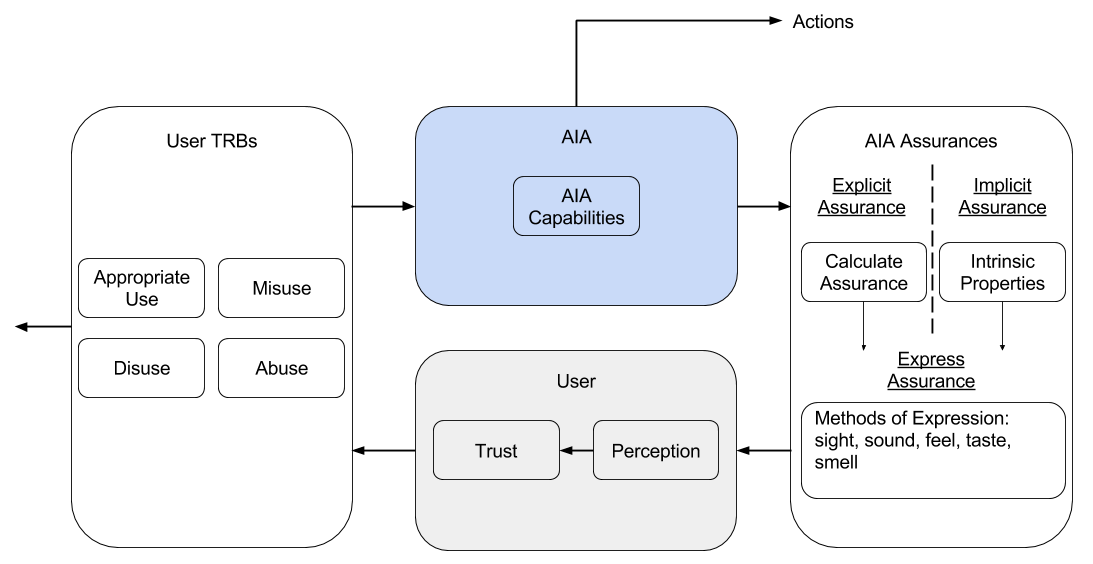
\includegraphics[width=0.85\textwidth]{Figures/RefinedTrust_one_way}
        \caption{Detailed extension of Figure~\ref{fig:SimpleTrust_one_way}. The AIA, User, and User TRBs blocks are defined as in Section~\ref{sec:background} (with the exception of the `Perception' blocks added to the AIA and User boxes). The AIA Assurances box has been filled using insights from the survey. The grey shaded boxes will not be discussed in this work; we focus on elements that a designer can address given an AIA with a fixed set of capabilities.}
        \label{fig:refined_assurances}
    \end{figure}

\subsubsection*{Survey Methodology} \label{sec:methodology}
    While theoretically a two-way trust model could be considered (i.e. in which the AIA also has trust in the user), attention is restricted here to a one-way trust relationship that considers only how user trust (and TRBs) evolves in response to assurances from the AIA. 

    It should be noted that it is practically impossible to perform a fully comprehensive survey of all AIA assurances, due to the broad spectrum of possible assurances, and AIAs in general. As an example, one could rightly argue that control engineers treat metrics like gain and phase margins as assurances for automatic feedback control systems, in much the same way that machine learning practitioners treat training and test accuracy as assurances for learning algorithms---and hence concepts related to robustness, stability, etc. for feedback control systems ought also be included in this survey. Similar arguments for assurances developed for fields like econometrics, software testing, aeronautical engineering and many others. While assurances can, in theory, be applied in both the most simple `automatic' systems (like a thermostat), this survey will focus on assurances in more advanced AIAs that make decisions under uncertainty. However, the admittedly narrow scope of this survey does not impede the development of fundamental insights and principles in designing assurances.

    Initially, in order to find applicable research, papers that formally addressed trust, and tried to create models of it, were investigated. This was done with the aim of trying to understand how trust might be influenced. Secondly, literature regarding trust between humans and some form of machine entity was reviewed; this lead to research in fields like e-commerce, automation, and human-robot interaction. Third, research on `interpretable', `comprehensible', `transparent', `explainable', and other similar types of learning and modeling methods were examined. Finally, with that literature as a background, research disciplines investigating computational methods that can be useful as assurances, but in which trust itself is not the main focus, were considered. This information was then used to construct an informed definition and classification of assurances based on methods that are currently in use, or being investigated.
    
    We now proceed to discuss each of the categories from Figure~\ref{fig:assurance_continuum}, starting from the most integral to the AIAs core functionality and proceeding to the least integral.

Recall that an assurance is defined as \emph{any} behavior or property of an AIA that affects a user's trust; an explicit assurance is any assurance that was consciously implemented/applied by the designer with the express intention of influencing a user's TRBs/trust (whether or not the means for doing so conforms to a formal trust concept). As such, it is possible to design assuring properties into the system a priori. It is likewise possible to design assuring behaviors into an AIA. From the literature, several key high-level issues emerge pertaining to assurance implementation: (1) uncertainty quantification; (2) complexity reduction; (3) assurance by design; and (4) planning strategies for assurances. 

\brettcomm{DISCUSS IMPLICIT VS EXPLICIT ASSURANCES HERE---PROBABLY SOMETHING LIKE A PARAGRAPH OR SO}

\begin{itemize}
    \item Quantifying Uncertainty
    \item Reducing Complexity
    \item Assurance by Design
    \item Planning Strategies of Assurance
\end{itemize}

\subsection{Quantifying Uncertainty} %%nra: awkward sentence: Being able to quantify the different kinds of uncertainty in the AIA is necessary before attempting to express that uncertainty to a human user. 
    An AIA must have some way to assess and quantify uncertainty before attempting to express those uncertainties to a human user. 
    There are several different kinds of uncertainty that might be considered, e.g. uncertainty in sensing, uncertainty in planning, and uncertainty in locomotion. 
    A model or method needs to be incorporated in the AIA that will represent the different kinds of uncertainty to the human user in some way. 
    A human user could use such information to inform their trust in the `situational normality', `competence', and/or `predictability' of the AIA. 
    One might imagine that, in the UGV road-network problem, the UGV expressing high uncertainty in its plan would influence the competence component of the user's trust. Conversely, if an uncertainty measure is not available, the user might take this as an implicit assurance that the AIA is perfectly confident, or (based on the user's experience)  might conclude that since all AIA plans have been flawed in the past, the plan of this AIA must be flawed as well. 

    The surveyed literature  featured several different uncertainty quantification approaches. In some cases uncertainty is already represented intrinsically by the algorithms and/or models being used in the AIA. Some use the built-in statistical representations of state transitions and sensor observations, e.g. for POMDPs, as the basis of quantifying uncertainty. This approach has straightforward analogs in other systems that use algorithms and/or models that inherently consider uncertainty. Models and methods that intrinsically represent uncertainty are frequently available. However, even when that it is the case, there are types of uncertainties that may still not be considered. For example, there are additional aspects of uncertainty beyond those intrinsically captured by some optimal planning approaches \cite{Aitken2016-cv,Kuter2015-qh}. 
    Using the UGV road network problem as an example, what is the total probability distribution over all possible total cumulative reward outcomes (i.e. beyond just the expected value maximized by the optimal policy)? 
    Or, given a certain road network, how closely can a Monte Carlo-based POMDP solver for the UGV approximate the true optimal policy? 
    These describe `uncertainties in application', which arise in applying certain algorithms and models in different contexts.

    Independent of the algorithms or representations used by an AIA, uncertainty quantification for assurance design also often focuses on assessing the probability of error for decision making as it pertains to any of the AIA capabilities from Fig. \ref{fig:AIcapabilities}. 
    %(regression methods have analogous approaches). 
    For instance, the problem of assessing the probability of error for classification and regression tasks for learning and perception are well-studied. 
    In addition to standard training/validation data-based assessment techniques, some have approached this problem by learning models of errors for underlying learning models, e.g. by training a GP error `meta-model' for classifier errors  from empirical training data and using the meta-model to quantify uncertainty in different test scenarios \cite{Gurau2016-hs}. 
    In contrast, we might quantify the uncertainty of a classifier based solely on the input data itself \cite{Zhang2014-he}. Of course, these methods share common drawbacks of being solely supervised learning approaches. However even in domains such as reinforcement learning, methods for avoiding highly uncertain (un-safe) rewards must use some form of external expert knowledge (see \cite{Garcia2015-rs, Lipton2016-dq}). Hence, the problem of defining a sensible `ground truth' against which uncertainties can be `correctly' assessed remains a fundamental challenge. %for developing AIA assurances.  
    %
    %\edit{...merge this paragraph with end of previous somehow...}
    %    Uncertainty can be easier to assess if some kind of oracle, or reference is available for comparison. 

    Some works have proposed quantifying the similarity between empirical experience and available reference data from a truth model as a measure of uncertainty \cite{Kaipa2015-hy}. Of course, this approach loses its appeal when a `truth model' isn't available. This shouldn't detract from the intent of finding some kind of reference (truth or otherwise) in which the reasoning, sensing, and other processes of an AIA can be compared to evaluate uncertainty. The evaluation of statistical models involves a very similar concept: given a statistical model as a reference does current empirical experience support or detract from the hypothesis that the model is still valid \cite{Laskey1995-jp,Ghosh2016-dl}? These approaches can quantify the degree to which the statistical models are still true, and this measurement can be used as an indication of uncertainty. However, these techniques can only provide binary indications that a model is statistically valid/invalid, without providing specific human-understandable causes or justifications as to why. Human expertise and designer judgment is thus required to carefully interpret such assurances, although a universal set of `best practices' for reporting such assurances and coping with cognitive biases in probabilistic/statistical data interpretation (framing effects, etc.) have yet to be established. 
    %
    %%This paragraph repeats the first one, so merging in the last part with that and commenting out the rest:
    %%Generally, uncertainty quantification allows AIAs to express assurances related to the `situational normality', `competence', and `predictability' of the system in a given situation. One might imagine that, in the UGV road-network problem, the UGV expressing high uncertainty in its plan would influence the competence component of the user's trust. Conversely, if an uncertainty measure is not available, the user might take this as an implicit assurance that the AIA is perfectly confident, or (based on the user's experience)  might conclude that since all AIA plans have been flawed in the past, the plan of this AIA must be flawed as well.
    %%
        \subsubsection{Reducing Complexity} Many researchers have attempted to remove complexity from the models and logic of the AIA to make the methods more interpretable (or comprehensible, or explainable, \ldots) to human users. 
    As with uncertainty quantification, interpretability can also inform a user's trust regarding the AIA's `situational normality', `competence', and `predictability'. Of course, this presupposes that many of the methods used by AIAs are `complex' by some measure; we claim that the fact that highly trained and educated experts are required to understand and develop these methods %(and even then it may not be totally possible) 
    proves this supposition. Complexity only exists in the presence of some reference frame, i.e. the designer's or the user's in this case. 
    From the perspective of an assurance designer, the key challenges to making/discovering/learning assurances with scalable interpretability lie in defining and satisfying criteria for required depth of understanding on the part of the user, the level of user expertise, and the time required by the user to gain understanding. 

    Generally, the `complexity' of an algorithm or more general process used by an AIA is said to increase with the number of variables, steps of reasoning, the size of data, etc. in the formal sense that is understood by computer scientists. 
    In practice, \textit{reduction} of complexity has been addressed by approaches as simple as finding summary statistics, e.g. calculating averages \cite{Muir1994-ow,Muir1996-gt}, that help explain why/how an algorithm or AIA arrives at a particular result. 
    This can also be accomplished by computing heuristic measures which reduce many complex algorithmic components into more manageable pieces\cite{Aitken2016-cv}. Creating variable fidelity models is another way by which complexity can be reduced (and increased when necessary). One might also elect to create and use models to support AIA reasoning, decision, making, etc. capabilities which are inherently more interpretable to humans. This could include constraining the feature space to be more simple, reducing dimensionality, learning more understandable features, and using physical theories to ground learned models (e.g. for interpretable science).  %%\edit{...merge? feels a bit out of place...}
        
    It is possible for `inherently interpretable models and algorithms' to compete with other non-interpretable models in terms of performance. 
    However, this may not be the most viable long-term approach for tackling the problem of complexity reduction in assurance design, especially due to the amount of work required to design interpretable counterparts to the latest state of the art algorithms for implementing AIA capabilities. 
    On the other hand, approaches that seek `post hoc' explanations of complex models and algorithms offer more promise. 
    This is partly because the idea of `interpretability' is not universally well-defined, and thus does not offer a single tangible goal. Rather, there exists a continuum of interpretability based on the complexity of the problem, the time required for a user to interpret (e.g. a few seconds vs. a few months of study, depending on the application), the expertise of the user, and other factors. However, assurances that can be automatically generated to provide user-specific and model/method-agnostic explanations/interpretations of complex AIA processes would provide the best of both worlds. These ideas are much more aligned with the efforts of \cite{Ruping2006-xj} and others who seek models with scalable resolution and accuracy.

\subsection{Assurance by Design}
    No matter how much engineers and system designers like to think about automating everything, humans will realistically need to be involved at some level of AIA operation as well as assurance design for the foreseeable future, since the human-AIA trust cycle cannot be properly managed without taking human inputs into consideration. 
    The problems of uncertainty quantification and complexity reduction can largely leverage existing methods to generate explicit assurances `on the fly' as needed for human users. 
    We have also seen that several strategies are available to directly engineer AIAs to be as meaningful and transparent to humans as possible from the outset through direct `consequential' forms of interaction. 

    One approach is to make the human user and human interpretability an intrinsic part of an AIA's decision making and learning processes, in order to modify their associated objective functions according to human user preferences \cite{Freitas2006-qo,Dragan2013-wd}. 
    Poorly designed objective functions are an important source of discord between how human users expect AIAs to behave and how AIAs actually behave (thus making them less predictable and less trustworthy) \cite{Amodei2016-xi}. 
    `Myopic objectives' are said to be present when an AIA focuses on a specific objective to the extent that a human can no longer relate to the objectives of the AIA (so that the user will be correspondingly surprised by its actions). This suggests that significant time may be required to design objectives that align with those of humans, in order to make the AIA more predictable, and competent in the user's eyes. 
    %
    `Human-in-the-loop' (HITL) methods can be used to implicitly encode many human qualities that cannot be expressly quantified or explained. 
    It is interesting to note that using HITL can offer more interpretability to the result of a learning process, while at the same time making the learning process itself less complex and procedural. 
    However, there are trade-offs that can be undesirable in many situations as well, as decision making and learning algorithms are often used to circumvent human biases and imperfect human reasoning. 

    Aside from relying on HITL, it is also possible to modify standard decision making and learning approaches (e.g. as discussed in the previous section) to make the methods inherently more transparent and assuring to users. For example, one might restructure a neural net architecture or a decision tree to make it more interpretable \cite{Choi2016-by,Abdollahi2016-vn,Jovanovic2016-gw}. However, there are no universally established principles yet for how this can/should be done.

\subsection{Planning Explicit Assurances}
    Computational resources are needed for an AIA to formulate and communicate assurances, as well as assess whether such assurances are eliciting the desired TRBs from users. This naturally raises the question of whether/how AIAs can formulate plans to achieve the goal of effectively and appropriately expressing assurances to a human user. 

    As mentioned earlier, not all AIAs are capable of planning. 
    Such AIAs can be designed beforehand with some kind of static plan or policy to deliver assurances (e.g. using a fixed set of rules). 
    Otherwise, more advanced AIAs might use TRBs as feedback signals to come up with assurance strategies designed to steer users into enacting appropriate TRBs. 

    When planning assurances, the AIA must be able to account for limitations of users, and its own limitations in expressing assurances. For example a user may not be able to understand information needed to use the AIA more appropriately. Also, the AIA may need to take a longer-term strategy to teach or tutor the user, as opposed to only presenting the user with canned, static, assurances. Some important user considerations are discussed in Section~\ref{sec:express_assurances}.
    
    One must ask whether the human user can correctly process the information received. This is perhaps most easily illustrated by considering a non-expert user who cannot understand highly technical assurances regarding the AIA. However, less trivial manifestations, such as the existence of bias in the perception of assurances, or the inability of users to recognize or process important information due to cognitive overload, are also possible. This will also be addressed in Section~\ref{sec:express_assurances}.

    The problem of planning for assurances is nearly unexplored in the context of human-AIA trust relationships. However, there are several fairly new research programs that are interested in this question (i.e. DARPA's Explainable Artificial Intelligence (XAI) program \cite{Gunning2016-kb}) and related ones (e.g. DARPA's Assured Autonomy program \cite{Neema2017-bb}). Assuming an AIA can provide assurances, important questions arise, such as: what is the best way to present them? How can they be adapted for different kinds of users? How can the AIA teach or tutor the human to use the AIA appropriately over time and in different operational contexts? The problem of enabling AIAs to be aware that they must take action and formulate plans to deliver assurances is a large gap in the current assurances landscape; answers to these questions are critical to designing more robust and effective assurances.



